\section{Views}
\label{sec:views}

\subsection{Logic View}
A simple version of the logic view was made because it is hard to foresee all
help classes and states prior to the start of the development process.
\begin{center}
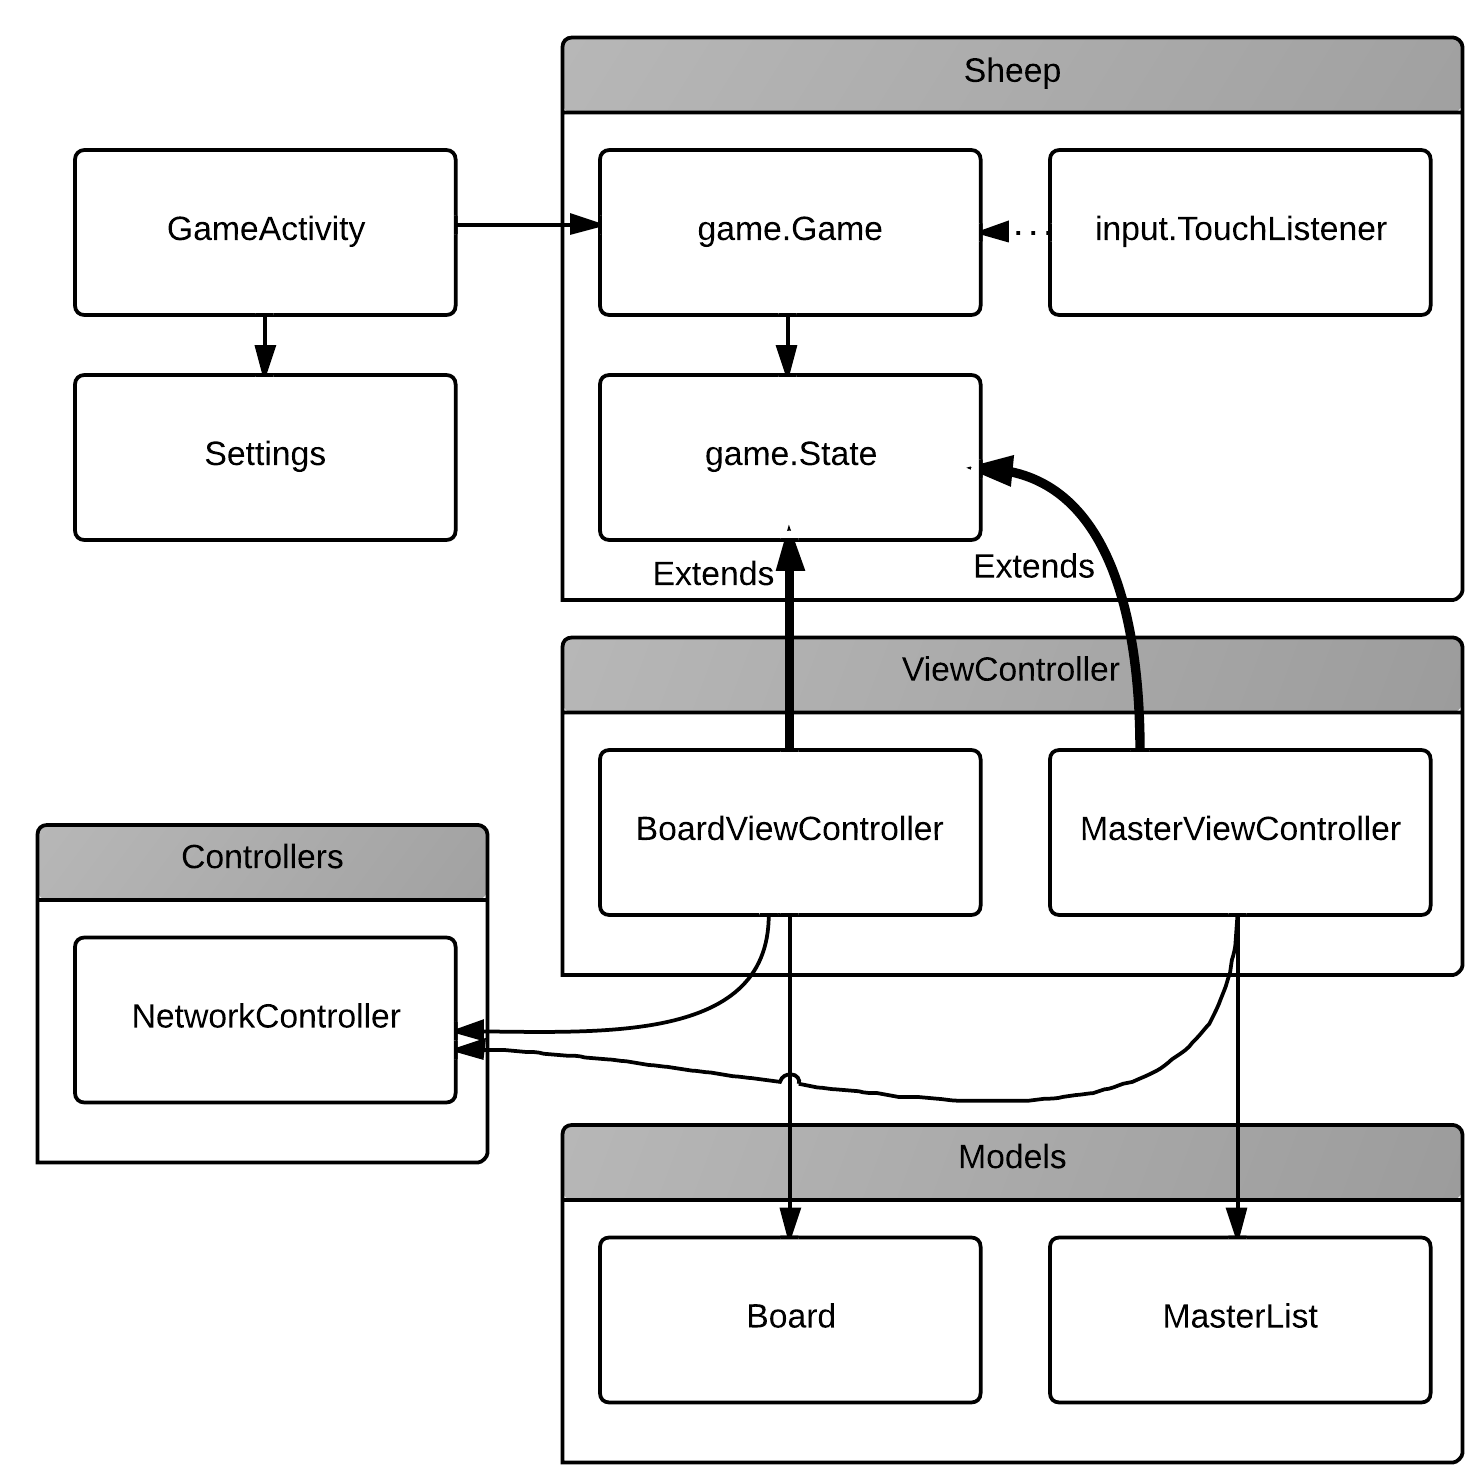
\includegraphics[clip=true, width=0.9 \textwidth]{assets/LogicView.png}
\captionof{figure}{Logic View}
\label{ref:gantt}
\end{center}

\subsection{Development View}
The development view is a hierarchy of layers containing assets such as the
graphics, the game logic (including handling of states and input), the Sheep
framework (which is a typical utility framework) and the Android SDK taking care
of the networking and the base communication with the Android platform.
\begin{center}
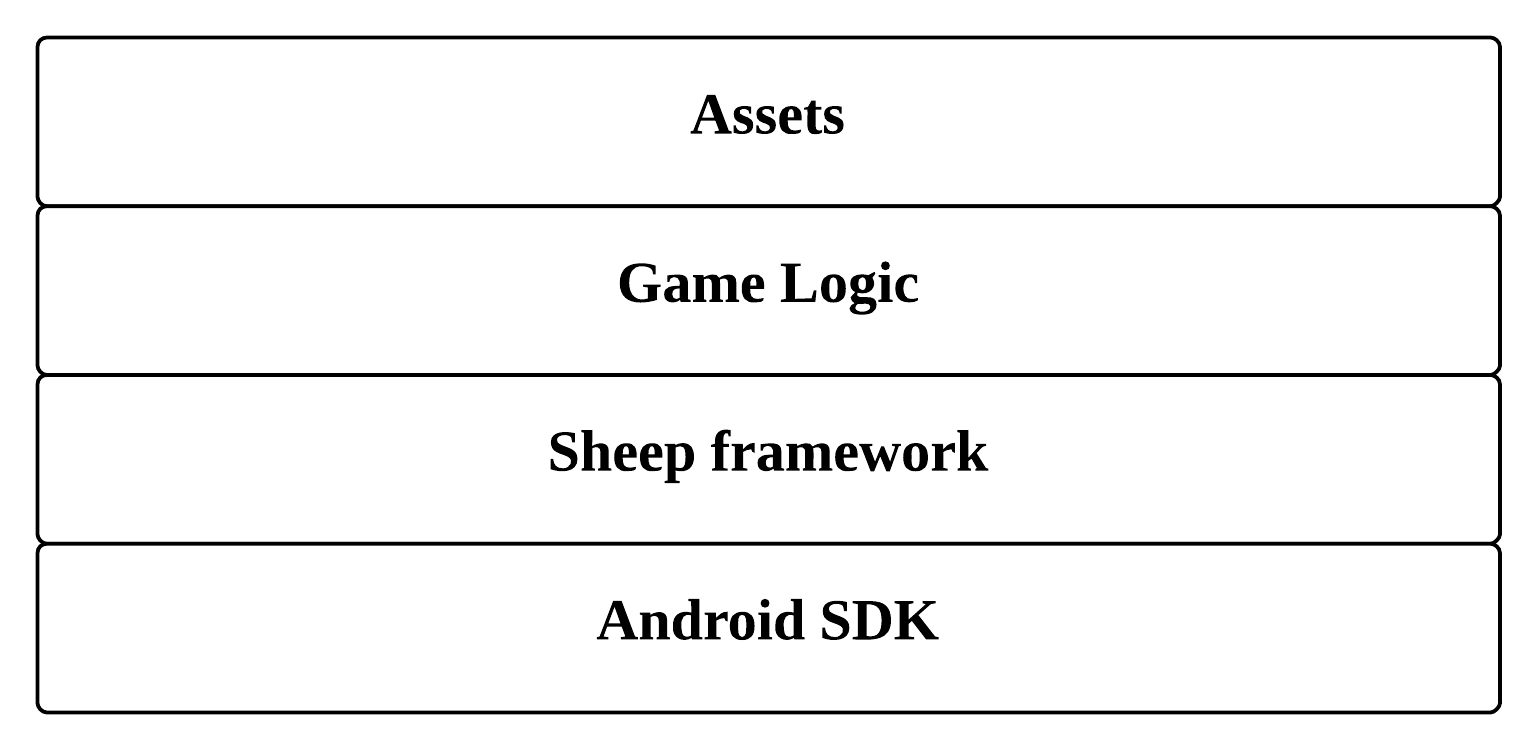
\includegraphics[clip=true, width=0.9 \textwidth]{assets/DevelopmentView.png}
\captionof{figure}{Development View}
\label{ref:gantt}
\end{center}

\subsection{Process View}
The process view shows the process flow in the game, how connections are made
between states and screens.

The menu screen is the entry point of this application where there are options
to navigate to either the authentication or the settings screens. From the
authentication screen the user can log in to, or out of, the admin screen.

The main menu also provides the option to join a new game. If this option is
chosen, the user is transferred to the game screen, which has listeners for
notification states. The game ended screen returns to the main menu.
\begin{center}
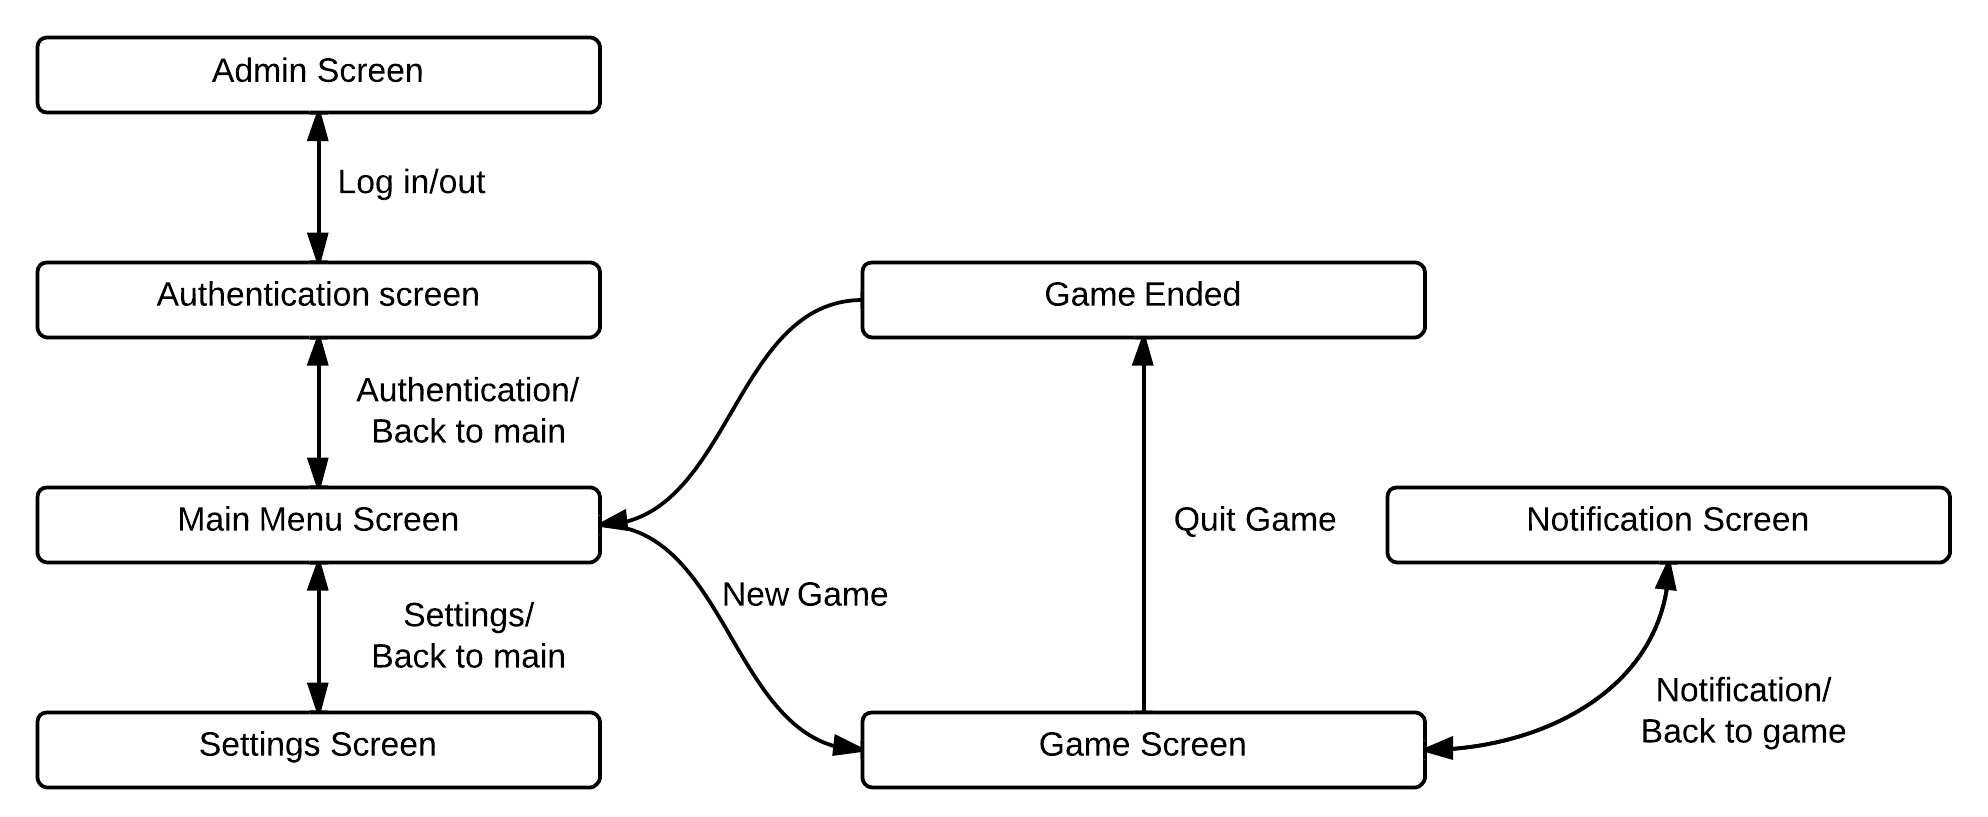
\includegraphics[clip=true, width=0.9 \textwidth]{assets/ProcessView.png}
\captionof{figure}{Process View}
\label{ref:gantt}
\end{center}

\subsection{Physical View}
The client is divided into the shuffled board, the game logic, game query and
the session info. The server includes the current words, which contain the
master list of words for the game, and returns a list of $n$ words (where
$n = x\times x$, and $x$ is the length and width of the game board) to the
shuffled board of the client. The game state is a two-way communication with
logic and the list of usable words. The connection pool relates to the session
info to ensure the connection between client and server is persistent, even
through disconnections.
\begin{center}
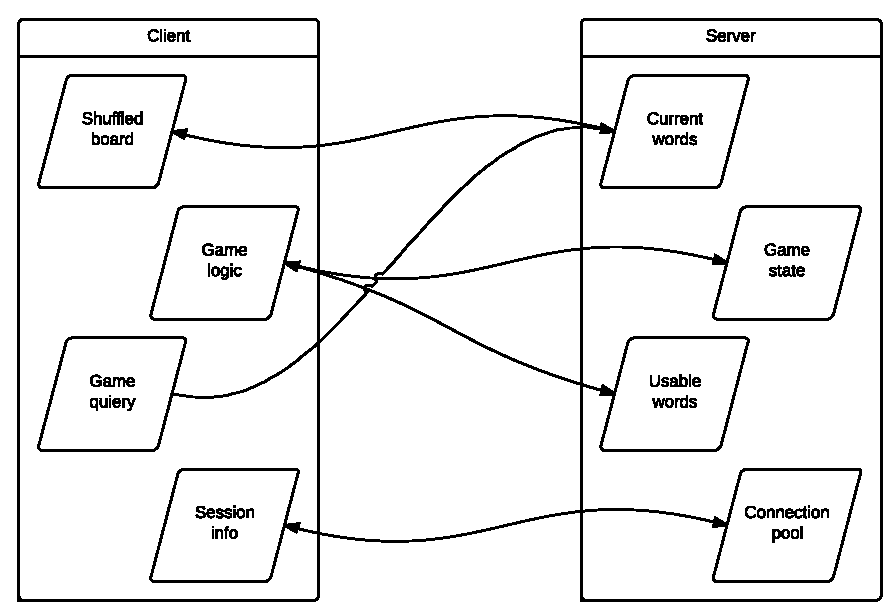
\includegraphics[clip=true, width=0.9 \textwidth]{assets/PhysicalView.pdf}
\captionof{figure}{Physical View}
\label{ref:gantt}
\end{center}

\subsection{Consistency among views} 
\label{sec:consistencyamongviews}
%TODO: Update when finished

Apart from the develompent view not showing specifically what goes under client
or server, the views are consistent. In the development view the server is
under the Game Logic, and networking is under the SDK\@.

Apart from this, the other views and relations are consistent.
